% Options for packages loaded elsewhere
\PassOptionsToPackage{unicode}{hyperref}
\PassOptionsToPackage{hyphens}{url}
\PassOptionsToPackage{dvipsnames,svgnames,x11names}{xcolor}
\documentclass[
  10pt,
  fontset=fandol]{ctexart}
\usepackage{xcolor}
\usepackage[margin=16mm]{geometry}
\usepackage{amsmath,amssymb}
\setcounter{secnumdepth}{-\maxdimen} % remove section numbering
\usepackage{iftex}
\ifPDFTeX
  \usepackage[T1]{fontenc}
  \usepackage[utf8]{inputenc}
  \usepackage{textcomp} % provide euro and other symbols
\else % if luatex or xetex
  \usepackage{unicode-math} % this also loads fontspec
  \defaultfontfeatures{Scale=MatchLowercase}
  \defaultfontfeatures[\rmfamily]{Ligatures=TeX,Scale=1}
\fi
\usepackage{lmodern}
\ifPDFTeX\else
  % xetex/luatex font selection
\fi
% Use upquote if available, for straight quotes in verbatim environments
\IfFileExists{upquote.sty}{\usepackage{upquote}}{}
\IfFileExists{microtype.sty}{% use microtype if available
  \usepackage[]{microtype}
  \UseMicrotypeSet[protrusion]{basicmath} % disable protrusion for tt fonts
}{}
\makeatletter
\@ifundefined{KOMAClassName}{% if non-KOMA class
  \IfFileExists{parskip.sty}{%
    \usepackage{parskip}
  }{% else
    \setlength{\parindent}{0pt}
    \setlength{\parskip}{6pt plus 2pt minus 1pt}}
}{% if KOMA class
  \KOMAoptions{parskip=half}}
\makeatother
\usepackage{longtable,booktabs,array}
\newcounter{none} % for unnumbered tables
\usepackage{calc} % for calculating minipage widths
% Correct order of tables after \paragraph or \subparagraph
\usepackage{etoolbox}
\makeatletter
\patchcmd\longtable{\par}{\if@noskipsec\mbox{}\fi\par}{}{}
\makeatother
% Allow footnotes in longtable head/foot
\IfFileExists{footnotehyper.sty}{\usepackage{footnotehyper}}{\usepackage{footnote}}
\makesavenoteenv{longtable}
\usepackage{graphicx}
\makeatletter
\newsavebox\pandoc@box
\newcommand*\pandocbounded[1]{% scales image to fit in text height/width
  \sbox\pandoc@box{#1}%
  \Gscale@div\@tempa{\textheight}{\dimexpr\ht\pandoc@box+\dp\pandoc@box\relax}%
  \Gscale@div\@tempb{\linewidth}{\wd\pandoc@box}%
  \ifdim\@tempb\p@<\@tempa\p@\let\@tempa\@tempb\fi% select the smaller of both
  \ifdim\@tempa\p@<\p@\scalebox{\@tempa}{\usebox\pandoc@box}%
  \else\usebox{\pandoc@box}%
  \fi%
}
% Set default figure placement to htbp
\def\fps@figure{htbp}
\makeatother
\setlength{\emergencystretch}{3em} % prevent overfull lines
\providecommand{\tightlist}{%
  \setlength{\itemsep}{0pt}\setlength{\parskip}{0pt}}
\usepackage{amsmath,amssymb,mathtools,needspace}
\xeCJKDeclareCharClass{CJK}{"2032,"0400->"04FF,"2160->"216B,"2460->"2473,"25A0,"25C7,"25CB,"25CF}
\IfFontExistsTF{Arial Unicode MS}{\xeCJKsetup{AutoFallBack=true}\setCJKfallbackfamilyfont{\CJKrmdefault}{Arial Unicode MS}}{}
\setcounter{secnumdepth}{0}
\setlength{\emergencystretch}{2em}
\allowdisplaybreaks
\usepackage{bookmark}
\IfFileExists{xurl.sty}{\usepackage{xurl}}{} % add URL line breaks if available
\urlstyle{same}
\hypersetup{
  pdftitle={相关链的二分手续},
  colorlinks=true,
  linkcolor={Maroon},
  filecolor={Maroon},
  citecolor={Blue},
  urlcolor={Blue},
  pdfcreator={LaTeX via pandoc}}

\title{相关链的二分手续}
\author{}
\date{}

\begin{document}
\maketitle

\subsubsection{11.3.1　相关链的二分手续}\label{ux76f8ux5173ux94feux7684ux4e8cux5206ux624bux7eed}

为了便于刻画二分法的设计思想，首先引进相关链的概念。由于递推关系式反映了变元之间的相关性和时序性，一组有序的相关变元可抽象地表述为如下形式的相关链：

\[
\cdots\to x_{i-j}\to x_i\to\cdots,
\]

其中相邻两元素 \(x_i\) 与 \(x_{i-j}\) 的下标之差 \(j\) 称作间距。如果相关链各节的间距为定值，则将其称作步长。

对应于递推问题（11.3.1）的相关链有 \(N\) 节，即

\[
x_0\to x_1\to\cdots\to x_{N-1},
\]

\href{../../source-images/pdf-286.jpeg}{原页图像}

这里步长等于 1。

设将上述相关链按其下标的奇偶拆成两条，则每条子链含 \(N_1=N/2\) 节，即

\[
\begin{cases}
x_0\to x_2\to\cdots\to x_{N-2},\\
x_1\to x_3\to\cdots\to x_{N-1}.
\end{cases}
\tag{11.3.2}
\]

这样加工得出的递推问题有两个结果 \(x_0,x_1\)，且其步长等于 2。这是一种二分手续。

在保持结果数逐步倍增及步长逐步倍增两项基本特征的前提下反复施行这一手续，则二分 \(k\) 次后得出 \(2^k\) 个结果 \(x_i\)，\(i=0,1,\cdots,2^k-1\)，且步长增至 \(2^k\)，相应地，所给相关链被加工成 \(2^k\) 条子链，每条子链含 \(N_k=N/2^k\) 节，即

\[
\left\{
\begin{aligned}
&x_0\to x_{2^k}\to\cdots\to x_{N-2^k},\\
&x_1\to x_{2^k+1}\to\cdots\to x_{N-2^k+1},\\
&\qquad\vdots\\
&x_{2^k-1}\to x_{2^{k+1}-1}\to\cdots\to x_{N-1}.
\end{aligned}
\right.
\tag{11.3.3}
\]

如此二分 \(n=\log_2 N\) 次后，所给相关链最终退化为每条仅含一节的最简形式

\[
x_0,x_1,\cdots,x_{N-1},
\]

从而得出所求的解。

这种以下标的奇偶分离为特征的二分手续称作奇偶二分。这是最基本的一种二分手续。

对于 \(N=8\) 的具体情形，相关链的奇偶二分过程如图 11.4 所示，图中用波纹线标出每一步的新结果。

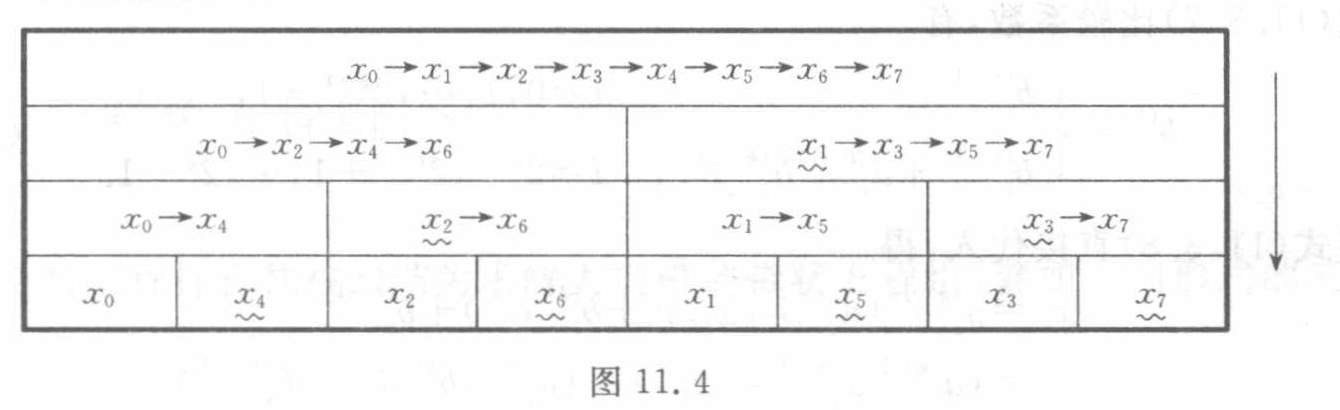
\includegraphics[width=0.85\linewidth,height=\textheight,keepaspectratio,alt={图 11.4（原图裁切）}]{../assets/ch11/figure-11-4.png}

图 11.4　原图右侧箭头向下，逐层由左至右的全部相关链与波纹线标记如下：

{\def\LTcaptype{none} % do not increment counter
\begin{longtable}[]{@{}
  >{\raggedright\arraybackslash}p{(\linewidth - 4\tabcolsep) * \real{0.3333}}
  >{\raggedright\arraybackslash}p{(\linewidth - 4\tabcolsep) * \real{0.3333}}
  >{\raggedright\arraybackslash}p{(\linewidth - 4\tabcolsep) * \real{0.3333}}@{}}
\toprule\noalign{}
\begin{minipage}[b]{\linewidth}\raggedright
层次（由上至下）
\end{minipage} & \begin{minipage}[b]{\linewidth}\raggedright
相关链或单节
\end{minipage} & \begin{minipage}[b]{\linewidth}\raggedright
波纹线标出的新结果
\end{minipage} \\
\midrule\noalign{}
\endhead
\bottomrule\noalign{}
\endlastfoot
初始层 & \(x_0\to x_1\to x_2\to x_3\to x_4\to x_5\to x_6\to x_7\) & 无 \\
第 1 次二分 & \(x_0\to x_2\to x_4\to x_6\)；\(x_1\to x_3\to x_5\to x_7\) & \(x_1\) \\
第 2 次二分 & \(x_0\to x_4\)；\(x_2\to x_6\)；\(x_1\to x_5\)；\(x_3\to x_7\) & \(x_2,x_3\) \\
第 3 次二分 & \(x_0\)；\(x_4\)；\(x_2\)；\(x_6\)；\(x_1\)；\(x_5\)；\(x_3\)；\(x_7\) & \(x_4,x_6,x_5,x_7\) \\
\end{longtable}
}

（上表为原图标签与结构的文字转录。）

\end{document}
